%----------------------------------------------------------------------------------------
%	PACKAGES AND THEMES
%----------------------------------------------------------------------------------------
\documentclass{beamer}
% Load a bunch of useful packages:
\usepackage{amssymb,amsmath,amsfonts,mathtools} % useful math fonts and symbols
\usepackage{geometry} % allows changing margins and sizes of stuff
\usepackage{hyperref} % allows referencing of lines of text, urls, figures etc
\usepackage{natbib} % allows citation referencing from a .bib file
\bibliographystyle{apalike} % American Psychological Association style guide
\usepackage{graphicx} % to include graphics from the figures folder with helpful formating options
\usepackage{tikz}
\usetikzlibrary{arrows}
\usepackage{pgfplots}
\usetikzlibrary{calc}
%---------------------------------------------%
\usepackage{color} % custom color definitions:%
    %UOregon colors:                          %
    \definecolor{UOGreen}{RGB}{18, 71, 52}    %
    \definecolor{UOYellow}{RGB}{254, 225, 35} %
    %Secondary official colors:               %
    \definecolor{LegacyGreen}{HTML}{104735}   %
    \definecolor{GrassGreen}{HTML}{489D46}    %
    \definecolor{LimeGreen}{HTML}{8ABB40}     %
    \definecolor{Chartreuse}{HTML}{E2E11B}    %
    \definecolor{Berry}{HTML}{8D1D58}         %
    \definecolor{DarkBlue}{HTML}{004F6E}      %
    \definecolor{LightBlue}{HTML}{00A5B5}     %
    \definecolor{crimson}{RGB}{ 170, 4, 36 }
    \definecolor{darkblue}{RGB}{ 4, 47, 170 }
    \definecolor{brown}{RGB}{ 111, 71, 2 }
    \definecolor{periwinkle}{RGB}{ 90, 177, 204 }
    \definecolor{ducksgreen}{HTML}{007030}
%----------------------------------------------

\usepackage{setspace} % to specify single, double or one-half spacing of text
\usepackage{indentfirst} % indent first line of a text paragraph
\usepackage{multicol} %multipage ability
\usepackage{multirow}
\usepackage{ulem} % \ul (underline) command which will break over line ends
\usepackage{amsthm} % allows standarized theorem commands
\setbeamertemplate{theorems}[numbered]
\theoremstyle{plain}
\newtheorem{assume}{Assumption}
\newtheorem{define}{Definition}
\usepackage{breqn} %automatic line breaking
\normalem

% Theming and Appearance Setup:
\usetheme{metropolis}
\metroset{block=fill}
%\usetheme{default}
\usefonttheme{professionalfonts}
\fontfamily{ppl}\selectfont
\usecolortheme[named=UOGreen]{structure}
\setbeamertemplate{footline}[frame number]
\setbeamertemplate{headline}{} %Removes Section Index on top of slide
\beamertemplatenavigationsymbolsempty
\hypersetup{
    colorlinks=true,
    linkcolor=DarkBlue,
    filecolor=Berry,
    citecolor=GrassGreen,
    urlcolor={LightBlue},
    pdftitle={Trade and Labor Market Dynamics},
    pdfpagemode=FullScreen
}

%----------------------------------------------------------------------------------------
%	TITLE PAGE
%----------------------------------------------------------------------------------------

% The title
\title{Mixed Strategies}
\author{Dante Yasui 
\\ adapted from material by Zachary Kiefer}
\institute{EC327 Game Theory}
\date{Winter 2024}
\titlegraphic{\includegraphics[scale=.4]{UOSignature-356.png}}


%-----------------------------------------------------------------------------
%	PRESENTATION SLIDES
%-----------------------------------------------------------------------------

\begin{document}

\begin{frame}[plain]
    % Print the title page as the first slide
    \titlepage
\end{frame}
\addtocounter{framenumber}{-1}

% \begin{frame}{Outline}
%   \tableofcontents
% \end{frame}

% - - - - - - - - - - - - - - - - - - - - - - - - - - - - - - - - - - - - - -
% \section{Uncertainty}

% 
% - - - - - - - - - - - - - - - - - - - - - - - - - - - - - -

\begin{frame}
\frametitle{Thinking about Randomness}
  \begin{quote}
    "I, at any rate, am convinced that [God] does not throw dice"
  \end{quote}

  - Albert Einstein 
  \footnote{1926, Letter to Max Born, published in 1971, Irene Born (translator), The Born-Einstein Letters, Walker and Company, New York}
\end{frame}

% - - - - - - - - - - - - - - - - - - - - - - - - - - - - - -

\begin{frame}{Thinking about Randomness}
  \begin{quote}
    "Rational decision makers are able to give reasons for each action they take;
    outside Las Vegas players do not spin roulette wheels"
  \end{quote}

  - Ariel Rubenstein
  \footnote{“John Nash: The Master of Economic Modeling.” The Scandinavian Journal of Economics 97, no. 1 (1995): 9–13. https://doi.org/10.2307/3440824.}
\end{frame}

% - - - - - - - - - - - - - - - - - - - - - - - - - - - - - -

\begin{frame}{Thinking about Randomness}
  
  Why should we use mixed strategies?!
  
  \begin{itemize}
    
    \item As we saw in Activity 2, 
    rarely do real life data fit in completely deterministic models

    \item You can interpret the mixed strategy of one player as the beliefs of other players in equilibrium

    \item Learning some basics of probability theory will help you outside of this class

  \end{itemize}
\end{frame}

% - - - - - - - - - - - - - - - - - - - - - - - - - - - - - -

\begin{frame}
\frametitle{Lotteries}
\begin{itemize}
  \item In this class, any choices with \textit{uncertain} payoffs will be called \alert{lotteries}.
	\item A lottery doesn't have to only be about money
  \item For any set of outcomes in a lottery, there will be an associated probability: if $a$ is a possible outcome, then $P(a)$ is the probability that it occurs.
	\begin{itemize}
		\item All probabilities must be between 0 and 1: $0 \leq P(a) \leq 1$ for all possibilities $a$.
		\item Additionally, the probabilities given in a particular lottery must sum to exactly 1: we will assume that one, and exactly one, outcome must actually occur.
	\end{itemize}
\end{itemize}
\end{frame}

% - - - - - - - - - - - - - - - - - - - - - - - - - - - - - -

\begin{frame}{Expected Utility}
  \begin{itemize}
    \item How can you know how much you like a given lottery
    if you don't even know what the outcome will be?

    \item A natural way would be to think of how happy it would make you \textit{on average}.

    \item The economists' term for this idea is 
    \alert{expected utility} or \alert{expected payoffs}.

  \end{itemize}
\end{frame}

% - - - - - - - - - - - - - - - - - - - - - - - - - - - - - -

\begin{frame}
\frametitle{Expected Payoffs}
\begin{itemize}
  \item You calculate an average by adding up the values of a lottery times the probability of how likely each is.
	\begin{itemize}
    \item $U(a) = \mathbb{E}[u(a)] = \sum_{a}u(a)P(a)$
	\end{itemize}
	\item This is a weighted average of the payoffs associated with each outcome $a$, with the weights being the probabilities of each one happening.
\end{itemize}
\end{frame}

% - - - - - - - - - - - - - - - - - - - - - - - - - - - - - -

\begin{frame}{Double or Nothing 'game'}
  \begin{figure}
    \includegraphics[width = .8\textwidth]{figures/doubleornothing.png}
  \end{figure}
\end{frame}

% - - - - - - - - - - - - - - - - - - - - - - - - - - - - - -

\begin{frame}
\frametitle{Expected Payoff Examples}
\begin{itemize}

  \item Zoidberg's expected payout if he Lets it Ride is 
	$0.50(\$10) + 0.50(\$0) = \$5 - \$0 = \$5$.

  \bigskip
	\item Let's face it, Zoidberg always has luck stacked against him, so suppose instead the coin has a 75\% probability of tails,
  \item The expected payoff would then be $0.25(\$10) + 0.75(\$0) = \$2.50 + \$0 = \$2.50 $.
\end{itemize}
\end{frame}

% - - - - - - - - - - - - - - - - - - - - - - - - - - - - - -

\begin{frame}
\frametitle{Test Your Understanding}
\begin{itemize}
	\item Suppose that you like sunny weather, and so you get payoff 5 when it is sunny, and -5 when it is rainy. There is a 10\% chance of rain and a 90\% chance of sun tomorrow. What is the expected payoff of this lottery?
	\begin{enumerate}
		\item -4.5
		\item -4
		\item 0
		\item 4
		\item 4.5
	\end{enumerate}
\end{itemize}
\end{frame}

% - - - - - - - - - - - - - - - - - - - - - - - - - - - - - -

\begin{frame}
\frametitle{Test Your Understanding}
\begin{itemize}
\item Suppose that in addition to a payoff of 5 when it is sunny and -5 when it is rainy, you get a payoff of 2 when it is overcast. There is a 40\% chance of rain, a 40\% chance of overcast, and a 20\% chance of sun tomorrow. What is the expected payoff of this lottery?
\begin{enumerate}
	\item -1.2
	\item -0.2
	\item 0
	\item 0.2
	\item 1.2
\end{enumerate}
\end{itemize}
\end{frame}

% - - - - - - - - - - - - - - - - - - - - - - - - - - - - - -

\begin{frame}
\frametitle{Cardinal Payoffs}
\begin{itemize}
\item Using expected payoffs implies that the payoffs of the outcomes are \alert{cardinal}, not merely ordinal: this means that the payoffs can be used not just to rank, but to compare the relative ``goodness" of outcomes.
\begin{itemize}
	\item i.e. an outcome with payoff 2 is actually twice as good as an outcome with payoff 1.
\end{itemize}
\end{itemize}
\end{frame}

\begin{frame}{Von-Neumann Morgenstern Utility}

  There are a few other axioms beyond just \textit{completeness} and \textit{transitivity}
  which are needed when it comes to making rational choices over lotteries.

  \begin{itemize}
    \item \alert{Continuity:} Small changes in lottery probabilities shouldn't make your ranking jump around.
    \item \alert{Independence:} If you know which of two lotteries you prefer, when I add a little bit of another unrelated option into both, it shouldn't change your mind.
  \end{itemize}

  Because \textit{expected utility} requires special assumptions beyond those of regular \textit{utility}, 
  it gets it's own special name: \\
  \alert{Von-Neumann Morgenstern utility function}
\end{frame}
% - - - - - - - - - - - - - - - - - - - - - - - - - - - - - -

\begin{frame}
\frametitle{Types of Uncertainty}
\begin{itemize}
	\item There are two main types of uncertainty that we'll cover in this course: \alert{external} and \alert{internal}.
	\item External uncertainty is the result of factors outside of the game, things that the players don't control, such as weather or other random events.
	\item Internal uncertainty is the result of the players' own actions inside of the game: it is caused whenever a player acts in a random way.
\end{itemize}
\end{frame}

% - - - - - - - - - - - - - - - - - - - - - - - - - - - - - -

\begin{frame}
\frametitle{External Uncertainty: States of Nature}
\begin{itemize}
\item The simplest form of uncertainty that we'll discuss is \underline{simple uncertainty}, or uncertainty about the \underline{state of nature}.
\item Under this form of uncertainty, the world may be in one of multiple states of nature, with the payoffs from each strategy profile being different in each state. 
\item Neither of the players know which state of nature is the correct one---but they do know the probability associated with each state.
\begin{itemize}
	\item The probability of each state must be between 0 and 1, and the sum of the probabilities of every state must sum to exactly 1, much like with lotteries.
\end{itemize}
\end{itemize}
\end{frame}

% - - - - - - - - - - - - - - - - - - - - - - - - - - - - - -

\begin{frame}
\frametitle{Example: A Card Game}
\begin{itemize}
\item Consider the following game, which models a very simple card game.
\item There are two players, Doc and Wyatt. Both are dealt a hand of cards: there is a 50\% probability that Wyatt's hand is better, and a 50\% probability that Doc's is. There are no ties.
\item At the beginning of the game, both players must bet \$1. 
\item After seeing his cards, Doc may either Stay, keeping the \$1 bet, or may Raise, bringing his bet to \$2.
\item Doc simultaneously decides to either Match Doc's bet, whatever that may be, or to Quit and forfeit his \$1.
\item If Wyatt Matches, the player with the better hand wins all the money. If Wyatt Quits, Doc wins all the money by default.
\end{itemize}
\end{frame}

% - - - - - - - - - - - - - - - - - - - - - - - - - - - - - -

\begin{frame}
\frametitle{Game Table: Doc's Hand is Better}
\begin{itemize}
\item In the state of nature where Doc has the better hand, this is the game table:
\end{itemize}
\begin{table}[h]
\centering
 
% - - - - - - - - - - - - - - - - - - - - - - - - - - - - - -

\begin{tabular}{cc|c|c|}
& \multicolumn{1}{c}{} & \multicolumn{2}{c}{Wyatt}\\
& \multicolumn{1}{c}{} & \multicolumn{1}{c}{$Match$}  & \multicolumn{1}{c}{$Quit$} \\\cline{3-4}
\multirow{2}*{Doc}  & $Stay$ & $1, -1$ & $1, -1$ \\\cline{3-4}
& $Raise$ & $2, -2$ & $1,-1$ \\\cline{3-4}
\end{tabular}
\end{table}
\end{frame}

\begin{frame}
\frametitle{Game Table: Wyatt's Hand is Better}
\begin{itemize}
\item On the other hand, if Wyatt has the better hand, this is the game table:
\end{itemize}
\begin{table}[h]
\centering
 
\begin{tabular}{cc|c|c|}
& \multicolumn{1}{c}{} & \multicolumn{2}{c}{Wyatt}\\
& \multicolumn{1}{c}{} & \multicolumn{1}{c}{$Match$}  & \multicolumn{1}{c}{$Quit$} \\\cline{3-4}
\multirow{2}*{Doc}  & $Stay$ & $-1, 1$ & $1, -1$ \\\cline{3-4}
& $Raise$ & $-2, 2$ & $1,-1$ \\\cline{3-4}
\end{tabular}
\end{table}
\end{frame}

\begin{frame}
\frametitle{Payoffs as Lotteries}
\begin{itemize}
\item We could easily solve each of these game tables to find the NE in either state of nature---but that doesn't matter, because neither player knows which state really applies. 
\item Instead, to solve this game, we must approach the payoffs as lotteries:
\begin{itemize}
\item Doc's payoff from strategy profile ($Stay,~Match$) is a lottery in which he gains 1 with probability 0.5, and loses 1 with probability 0.5.
\item Wyatt's payoff from the same strategy profile is a lottery in which he loses 1 with probability 0.5, and gains 1 with probability 0.5.
\item the expected payoffs of these lotteries are both 0. 
\end{itemize}
\item We can find the expected payoffs associated with each other strategy profile in the same way.
\end{itemize}
\end{frame}

\begin{frame}
\frametitle{Game Table: Expected Payoffs}
\begin{table}[h]
\centering
 
\begin{tabular}{cc|c|c|}
& \multicolumn{1}{c}{} & \multicolumn{2}{c}{Wyatt}\\
& \multicolumn{1}{c}{} & \multicolumn{1}{c}{$Match$}  & \multicolumn{1}{c}{$Quit$} \\\cline{3-4}
\multirow{2}*{Doc}  & $Stay$ & $0, 0$ & $1, -1$ \\\cline{3-4}
& $Raise$ & $0, 0$ & $1,-1$ \\\cline{3-4}
\end{tabular}
\end{table}
\begin{itemize}
\item It is trivial to see that the Nash equilibria of this game under uncertainty are ($Stay,~Match$) and ($Raise,~Match$).
\end{itemize}
\end{frame}

% - - - - - - - - - - - - - - - - - - - - - - - - - - - - - -

\begin{frame}
\frametitle{Example: The Deer Hunt with Randomness}
\begin{itemize}
\item Consider a variant of the Deer Hunt game, in which the success of the hunt is random.
\item Regardless of what Igg and Ogg decide to hunt, there is a 1/3\% probability that there are simply no Deer or Rabbits to be caught, and a 1/6 probability that the Rabbits are four times as plentiful.
\item This can be modeled as a game with three states of nature.
\end{itemize}
\end{frame}

% - - - - - - - - - - - - - - - - - - - - - - - - - - - - - -

\begin{frame}
\frametitle{Game Table: Normal Wildlife}
\begin{itemize}
\item In the normal state of nature, which occurs with probability 1/2, we have the normal Deer Hunt:
\end{itemize}
\begin{table}[h]
\centering
 
% - - - - - - - - - - - - - - - - - - - - - - - - - - - - - -

\begin{tabular}{cc|c|c|}
	& \multicolumn{1}{c}{} & \multicolumn{2}{c}{Ogg}\\
	& \multicolumn{1}{c}{} & \multicolumn{1}{c}{$Deer$}  & \multicolumn{1}{c}{$Rabbit$} \\\cline{3-4}
	\multirow{2}*{Igg}  & $Deer$ & $2, 2$ & $0, 1$ \\\cline{3-4}
	& $Rabbit$ & $1, 0$ & $1, 1$ \\\cline{3-4}
\end{tabular}
\end{table}
\end{frame}

% - - - - - - - - - - - - - - - - - - - - - - - - - - - - - -

\begin{frame}
\frametitle{Game Table: No Animals}
\begin{itemize}
\item With 1/3 probability, there are no animals to catch:
\end{itemize}
\begin{table}[h]
\centering
 
% - - - - - - - - - - - - - - - - - - - - - - - - - - - - - -

\begin{tabular}{cc|c|c|}
	& \multicolumn{1}{c}{} & \multicolumn{2}{c}{Ogg}\\
	& \multicolumn{1}{c}{} & \multicolumn{1}{c}{$Deer$}  & \multicolumn{1}{c}{$Rabbit$} \\\cline{3-4}
	\multirow{2}*{Igg}  & $Deer$ & $0, 0$ & $0, 0$ \\\cline{3-4}
	& $Rabbit$ & $0, 0$ & $0, 0$ \\\cline{3-4}
\end{tabular}
\end{table}
\end{frame}

% - - - - - - - - - - - - - - - - - - - - - - - - - - - - - -

\begin{frame}
\frametitle{Game Table: Abundant Rabbits}
\begin{itemize}
\item With 1/6 probability, there are very high payoffs from hunting Rabbits:
\end{itemize}
\begin{table}[h]
\centering
 
% - - - - - - - - - - - - - - - - - - - - - - - - - - - - - -

\begin{tabular}{cc|c|c|}
	& \multicolumn{1}{c}{} & \multicolumn{2}{c}{Ogg}\\
	& \multicolumn{1}{c}{} & \multicolumn{1}{c}{$Deer$}  & \multicolumn{1}{c}{$Rabbit$} \\\cline{3-4}
	\multirow{2}*{Igg}  & $Deer$ & $2, 2$ & $0, 4$ \\\cline{3-4}
	& $Rabbit$ & $4, 0$ & $4, 4$ \\\cline{3-4}
\end{tabular}
\end{table}
\end{frame}

% - - - - - - - - - - - - - - - - - - - - - - - - - - - - - -

\begin{frame}
\frametitle{Payoffs as Lotteries}
\begin{itemize}
\item There is a convenient shorthand for finding the expected payoffs to the game:
\begin{itemize}
\item (Deer, Deer): $1/2(2, 2) + 1/3(0, 0) + 1/6(2, 2) = (1, 1) + (0, 0) + (1/3, 1/3) = (4/3, 4/3)$.
\item (Deer, Rabbit): $1/2(0, 1) + 1/3(0, 0) + 1/6(0, 4) = (0, 1/2) + (0, 0) + (0, 2/3) = (0, 7/6)$.
\item (Rabbit, Deer): $1/2(1, 0) + 1/3(0, 0) + 1/6(4, 0) = (1/2, 0) + (0, 0) + (2/3, 0) = (7/6, 0)$.
\item (Rabbit, Rabbit): $1/2(1, 1) + 1/3(0, 0) + 1/6(4, 4) = (1/2, 1/2) + (0, 0) + (2/3, 2/3) = (7/6, 7/6)$.
\end{itemize}
\end{itemize}
\end{frame}

% - - - - - - - - - - - - - - - - - - - - - - - - - - - - - -

\begin{frame}
\frametitle{Game Table: Expected Payoffs}
\begin{table}[h]
	\centering
	\begin{tabular}{cc|c|c|}
		& \multicolumn{1}{c}{} & \multicolumn{2}{c}{Ogg}\\
		& \multicolumn{1}{c}{} & \multicolumn{1}{c}{$Deer$}  & \multicolumn{1}{c}{$Rabbit$} \\\cline{3-4}
		\multirow{2}*{Igg}  & $Deer$ & $4/3, 4/3$ & $0, 7/6$ \\\cline{3-4}
		& $Rabbit$ & $7/6, 0$ & $7/6, 7/6$ \\\cline{3-4}
	\end{tabular}
\end{table}
\begin{itemize}
\item Despite the introduction of randomness into this game, the Nash equilibria remain (Deer, Deer) and (Rabbit, Rabbit).
\end{itemize}
\end{frame}

% - - - - - - - - - - - - - - - - - - - - - - - - - - - - - -

\begin{frame}
\frametitle{iClicker Q3}
\begin{itemize}
\item Consider the following game with two states of nature. What are Player 1 and Player 2's expected payoffs from the strategy profile $(South, Split)$? (Choices on next slide.)
\end{itemize}
\begin{table}[h]
\begin{minipage}{0.49\linewidth}
	\centering
	\textbf{Sunny ($p = \frac{1}{3}$)}\\
	\begin{tabular}{cc|c|c|}
		& \multicolumn{1}{c}{} & \multicolumn{2}{c}{Player 2}\\
		& \multicolumn{1}{c}{} & \multicolumn{1}{c}{$Join$}  & \multicolumn{1}{c}{$Split$} \\\cline{3-4}
		\multirow{2}*{Player 1}  & $North$ & $5, 2$ & $1, 1$ \\\cline{3-4}
		& $South$ & $0, 0$ & $2, 5$ \\\cline{3-4}
	\end{tabular}
\end{minipage}
\begin{minipage}{0.49\linewidth}
	\centering
	\textbf{Rainy ($p = \frac{2}{3}$)}\\
	\begin{tabular}{cc|c|c|}
		& \multicolumn{1}{c}{} & \multicolumn{2}{c}{Player 2}\\
		& \multicolumn{1}{c}{} & \multicolumn{1}{c}{$Join$}  & \multicolumn{1}{c}{$Split$} \\\cline{3-4}
		\multirow{2}*{Player 1}  & $North$ & $2, 5$ & $0, 0$ \\\cline{3-4}
		& $South$ & $1, 1$ & $5, 2$ \\\cline{3-4}
	\end{tabular}
\end{minipage}
\end{table}
\end{frame}

% - - - - - - - - - - - - - - - - - - - - - - - - - - - - - -

\begin{frame}
\frametitle{iClicker Q3}
\begin{itemize}
\item What are Player 1 and Player 2's expected payoffs from the strategy profile $(South, Split)$?
\begin{enumerate}
\item (3, 3)
\item (3, 4)
\item (4, 3)
\item (4, 4)
\item (5, 2)
\end{enumerate}
\end{itemize}
\end{frame}

% - - - - - - - - - - - - - - - - - - - - - - - - - - - - - -

\begin{frame}
\frametitle{Variation: Unknown Probabilities}
\begin{itemize}
\item Suppose that the probability Doc has the better hand is $p$, and the probability Wyatt has the better hand is therefore $1 - p$. How large does $p$ have to be before there is a Nash equilibrium where Wyatt Quits?
\begin{itemize}
	\item We can find the expected payoffs in terms of p:
	\item (Stay, Match):
	\begin{itemize}
		\item Doc's Expected Payoff: $1(p) + -1(1 - p) = p - 1 + p = 2p - 1$.
		\item Wyatt's Expected Payoff: $-1(p) + 1(1 - p) = -p + 1 - p = 1 - 2p$.
	\end{itemize}
\end{itemize}
\end{itemize}
\end{frame}

% - - - - - - - - - - - - - - - - - - - - - - - - - - - - - -

\begin{frame}
\frametitle{Variation: Unknown Probabilities}
\begin{itemize}
	\item (Raise, Match):
	\begin{itemize}
		\item Doc's Expected Payoff: $2(p) + -2(1 - p) = 2p - 2 + 2p = 4p - 2$.
		\item Wyatt's Expected Payoff: $-2(p) + 2(1 - p) = -2p + 2 - 2p = 2 - 4p$.
	\end{itemize}
	\item (Stay, Quit) and (Raise, Quit):
	\begin{itemize}
		\item If Wyatt Quits, it doesn't matter who has the better hand: Wyatt loses the \$1 he bet already, and Doc gets it. The expected payoffs here are just (1, -1).
	\end{itemize}
\end{itemize}
\end{frame}

% - - - - - - - - - - - - - - - - - - - - - - - - - - - - - -

\begin{frame}
\frametitle{Variation: Unknown Probabilities}
\begin{table}[h]
\centering
\begin{tabular}{cc|c|c|}
& \multicolumn{1}{c}{} & \multicolumn{2}{c}{Wyatt}\\
& \multicolumn{1}{c}{} & \multicolumn{1}{c}{$Match$}  & \multicolumn{1}{c}{$Quit$} \\\cline{3-4}
\multirow{2}*{Doc}  & $Stay$ & $2p - 1, 1 - 2p$ & $1, -1$ \\\cline{3-4}
& $Raise$ & $4p - 2, 2 - 4p$ & $1,-1$ \\\cline{3-4}
\end{tabular}
\end{table}
\begin{itemize}
\item If Wyatt Quits, Doc doesn't care whether he Stays or Raises---he gets 1 either way. To have a NE where Wyatt Quits, we just need Wyatt to be happy with Quitting.
\item ($Stay,~Quit$) is a NE if $-1 \geq 1 - 2p$, i.e. if $p \geq 1$.
\item ($Raise,~Quit$) is a NE if $-1 \geq 2 - 4p$, i.e. if $p \geq \frac{3}{4}$.
\item One interpretation of this is that it is only rational for Wyatt to Quit if he is very confident that Doc has the better hand.
\end{itemize}
\end{frame}

% - - - - - - - - - - - - - - - - - - - - - - - - - - - - - -

\begin{frame}
\frametitle{Variation: Sequential Moves}
\begin{itemize}
\item It's not realistic to have Doc and Wyatt move at the same time: in actual card games, Doc would decide whether to raise, and Wyatt would then see that move and decide whether to match or quit.
\item So let's model this as an extensive-form game and make a game tree:
\end{itemize}
\end{frame}

\begin{frame}
\frametitle{Sequential Card Game Tree}
% \begin{figure}
% \centering
% \includegraphics[width=\textwidth]{Images/08SequentialCards.png}
% \end{figure}
\end{frame}

\begin{frame}
\frametitle{Information Sets in the Sequential Card Game}
\begin{itemize}
\item The dashed lines in this game tree denote information sets, showing that neither player knows the state of nature---however, Wyatt does know whether Doc chose to Stay or Raise.
\item When Doc and Wyatt reach one of their information sets, they don't know which of its nodes they're actually at, but in this case, because the node is determined by the state of nature, they know the probabilities of each node.
\item Once again, we can find the expected payoffs associated with each strategy profile. In fact, they're the same payoffs that we had in the strategic-form game---we just need to fit them into a game tree.
\end{itemize}
\end{frame}

\begin{frame}
\frametitle{Expected Payoff Game Tree}
% \begin{figure}
% \centering
% \includegraphics[width=\textwidth]{Images/08SequentialCardsVNM.png}
% \end{figure}
\end{frame}

\begin{frame}
\frametitle{SPNE in the Sequential-Move Card Game}
\begin{itemize}
	\item Let's look for SPNEs in this game---they will depend on what p is.
	\item A good place to start is with \alert{indifference points}, or values of p that make the players indifferent between their choices. Let's look at Wyatt's decisions:
	\begin{itemize}
		\item In the left-hand subgame (after Doc Stays), Wyatt has the choice between $1 - 2p$ and $-1$. Indifference implies that $1 - 2p = -1$, or $p = 1$. Wyatt is only indifferent here if Doc is guaranteed to have the better hand; if $p < 1$, Wyatt will simply prefer to Match.
		\item In the right-hand subgame (after Doc Raises), $2 - 4p = -1$ implies $p = \frac{3}{4}$. If $p < \frac{3}{4}$, Wyatt will prefer to Match; if $p > \frac{3}{4}$, Wyatt will prefer to Quit.
	\end{itemize}
	\item It may help to plot this on a number line...
\end{itemize}
\end{frame}

\begin{frame}
\frametitle{SPNE in the Sequential-Move Card Game}
\begin{itemize}
	\item Now let's consider Doc's decisions:
	\begin{itemize}
		\item If Wyatt plays (Match, Match), implying that $p \leq \frac{3}{4}$, Doc's choice is between $2p-1$ and $4p-2$. Doc is indifferent when $p = \frac{1}{2}$; when p is smaller, he prefers to Stay, and when p is larger, he prefers to Raise.
		\item If Wyatt plays (Match, Quit), implying that $\frac{3}{4} \leq p \leq 1$, Doc's choice is between $2p - 1$ and $1$. Doc is indifferent if $p = 1$; for $\frac{3}{4} \leq p < 1$, Doc prefers to Raise.
		\item If Wyatt plays (Quit, Quit), which he would only do if $p = 1$ exactly, Doc's choice is between $-1$ and $-1$: not really a choice at all. Doc is completely indifferent here.
	\end{itemize}
\end{itemize}
\end{frame}

\begin{frame}
\frametitle{Plotting SPNEs}
\end{frame}

\begin{frame}
\frametitle{Summary of SPNE in Sequential-Move Card Game}
\begin{itemize}
\item We can summarize all of the possible SPNEs as follows:
\begin{itemize}
\item \{Stay, (Match, Match)\} is an SPNE if $0 \leq p \leq \frac{1}{2}$.
\item \{Raise, (Match, Match)\} is an SPNE if $\frac{1}{2} \leq p \leq \frac{3}{4}$.
\item \{Raise, (Match, Quit)\} is an SPNE if $\frac{3}{4} \leq p \leq 1$.
\item \{Stay, (Match, Quit)\}, \{Stay, (Quit, Quit)\}, and \{Raise, (Quit, Quit)\} are all SPNEs if $p = 1$.
\end{itemize}
\end{itemize}
\end{frame}



\section{Mixed Strategies}


\begin{frame}
\frametitle{Internal Uncertainty}
\begin{itemize}
  
  \item Now that we discussed \textit{external uncertainty} over \textit{states of nature},
  let's talk about \alert{internal uncertainty}.

	\item Internal uncertainty occurs when one or more players pick their strategies randomly.

	\item Picking a strategy at random is really just a different kind of strategy, called a \alert{mixed strategy}.
\end{itemize}
\end{frame}

\begin{frame}
\frametitle{Mixed Strategies}
\begin{itemize}

	\item When a player always does the same thing, it's called a \alert{pure strategy}.
  
  \item A \alert{mixed strategy} assigns a probability to each of a player's pure strategies. 

  \begin{itemize}
    \item Like a lottery, the probabilities in a mixed strategy must all be between 0 and 1,
    \item and must sum to exactly 1.
  \end{itemize}
\end{itemize}
\end{frame}

\begin{frame}{Mixed Strategies}

\begin{itemize}

  \item A mixed strategy can assign 0 probability to a pure strategy.

  \item It can even assign probability 1 to a single pure strategy, and probability 0 to all others
  
  \begin{itemize}
    \item this is still, technically, a mixed strategy, but it is a trivial one.
  \end{itemize}

	\item When a player uses a mixed strategy, it turns the \textbf{other} player's payoffs into lotteries.
  
\end{itemize}
\end{frame}

\begin{frame}
\frametitle{Mixed Strategies in the Deer Hunt}

Consider the Deer Hunt:

\begin{table}[h]
\centering
\begin{tabular}{cc|c|c|}
	& \multicolumn{1}{c}{} & \multicolumn{2}{c}{Ogg}\\
	& \multicolumn{1}{c}{} & \multicolumn{1}{c}{$Deer$}  & \multicolumn{1}{c}{$Rabbit$} \\\cline{3-4}
	\multirow{2}*{Igg}  & $Deer$ & $2, 2$ & $0, 1$ \\\cline{3-4}
	& $Rabbit$ & $1, 0$ & $1, 1$ \\\cline{3-4}
\end{tabular}
\end{table}

\begin{itemize}
	\item Suppose that Igg hunts Deer 3/4 of the time, and Rabbit 1/4 of the time.

  \item If Ogg \textit{always hunts deer}; 
  what is Ogg's \textit{expected payoff}?

  \vspace{5mm}

	% \item Ogg's expected payoff from playing Deer will be $0.75(2) + 0.25(0) = 1.5$.
\end{itemize}
\end{frame}

\begin{frame}
\frametitle{Mixed Strategies in the Deer Hunt: Generalizing}

We can generalize this approach to calculate Ogg's expected payoffs from any strategy that Igg chooses to play:

\begin{itemize}

	\item Suppose that Igg plays Deer with probability p, and Rabbit with probability 1 - p.

	\item Then Ogg's expected payoff from Deer is:
  % $2(p) + 0(1 - p) = 2p$, and from Rabbit, it is $1(p) + 1(1 - p) = 1$.
  \vspace{20mm}

	\item Note that Ogg's expected payoff from Deer gets larger with p: the more likely Igg is to hunt Deer, the more attractive an option it becomes for Ogg.

\end{itemize}
\end{frame}

\begin{frame}
\frametitle{When to Play a Mixed Strategy?}
\begin{itemize}

	\item It's possible for a mixed strategy to be a best response to the other player's strategy:

  \begin{itemize}
    \item if and only if all of the mixed strategy's \alert{components} (pure strategies that are assigned positive probability) are best responses too.
  \end{itemize}

	\item Some intuition: If a strategy is not a best response, you should not play it---even as part of a mixed strategy.

\end{itemize}
\end{frame}

\begin{frame}{When to play a Mixed Strategy?}

  If a player only has \textbf{two pure strategies}, it becomes simple to tell when a mixed strategy is a best response: the mixed strategy must be a mixture of those two pure strategies, and the only way that both of them are best responses is if they have equal expected payoffs.

\begin{itemize}
	\item Taking the Deer Hunt as an example, the only way that it can be a best response for Ogg to play a mixed strategy is if Deer and Rabbit provide Ogg with equal expected payoffs: we must have $2p = 1$, or $p = \frac{1}{2}$.
\end{itemize}
\end{frame}

% \begin{frame}
% \frametitle{What Mixed Strategy to Play}
% \begin{itemize}
% 	\item However, if any mixed strategy is a best response, then \textbf{all} mixed strategies (with the same components) are also best responses.
% 	\item Intuitively, if the pure strategies going into a mixed strategy are just as good as each other, then it doesn't matter what proportions you mix them in.
% 	\item This means that, while it's easy to solve for \textbf{when} it's rational for a player to use a mixed strategy, there's no way to solve for a particular mixed strategy that the player \textbf{should} play.
% \end{itemize}
% \end{frame}

\begin{frame}
\frametitle{Mixed-Strategy Nash Equilibrium}
	To solve for the Nash equilibria where players are allowed to use mixed strategies:

  we need to look for the conditions under which a player would be willing to use a mixed strategy.

\begin{itemize}

	\item This means that we're going to use one player's expected payoffs to solve for the \textbf{other} player's mixed strategy

\end{itemize}
\end{frame}

\begin{frame}
\frametitle{MSNE in the Deer Hunt}
\begin{itemize}
	\item Returning to the Deer Hunt, let's say that Igg plays Deer with probability $p$ and Rabbit with probability $1 - p$...
	\item While Ogg plays Deer with probability $q$ and Rabbit with probability $1 - q$.
	\begin{itemize}
		\item This is simply a framework for describing each player's mixed strategies:
    we're using placeholder variables for the players' mixed strategy probabilities
	\end{itemize}
\end{itemize}
\end{frame}

\begin{frame}{MSNE in the Deer Hunt}
  \begin{itemize}
	\item We already saw that Ogg's expected payoffs from Deer and Rabbit are $2p$ and $1$, respectively, 
    so Ogg would only play a mixed strategy if $p = \frac{1}{2}$.

	\item Likewise, Igg's expected payoffs are $2q$ and $1$, and Igg will play a mixed strategy if $q = \frac{1}{2}$.

	\item The MSNE in this game can be written as:

    $$ \{(1/2~Deer, 1/2~Rabbit)_{Ogg}, \ (1/2~Deer, 1/2~Rabbit)_{Igg}\}$$.

\end{itemize}
\end{frame}

% \begin{frame}
% 
%   Another way to write out mixed strategies using $\sigma$:
% 
%   $$ \sigma_{Ogg} =  
% \end{frame}

\begin{frame}
\frametitle{Error-Checking}
\begin{itemize}
	\item Make sure that you're setting up the equations used to solve for a player's strategy correctly:
	\begin{itemize}
		\item Remember that you are creating an equation to describe when a player is indifferent between their pure strategies: if you're trying to figure out when \textbf{Player 1} is indifferent, you need to use \textbf{Player 1's} payoffs.
		\item However, when calculating expected payoffs, the probabilities will be based on the \textbf{other} player's mixed strategy: in a game with mixed strategies, the randomness a player deals with is created by the \textbf{other} player---not themselves.
	\end{itemize}
\end{itemize}
\end{frame}

\begin{frame}
\frametitle{Another Example: Police Patrol and Drug Trade
  \footnote{Harrington, pg. 226}}
\begin{table}[h]
	\centering
	\begin{tabular}{cc|c|c|}
		& \multicolumn{1}{c}{} & \multicolumn{2}{c}{Drug Dealer}\\
		& \multicolumn{1}{c}{} & \multicolumn{1}{c}{Streets (d)}  & \multicolumn{1}{c}{Park (1 - d)} \\\cline{3-4}
		\multirow{2}*{Police}  & Streets (p) & 80, 20 & 0,100 \\\cline{3-4}
		& Park (1 - p) & 10,90 & 60,40 \\\cline{3-4}
	\end{tabular}
\end{table}
\begin{itemize}
	\item Police Officer's expected utility:
  % $U_B(Bach) = 3q + 0(1 - q) = 3q$ and $U_B(Strav.) = 0q + 2(1 - q) = 2 - 2q$.
  \vspace{15mm}
	\item Drug Dealer's expected utility:
  % $U_S(Bach) = 2p$ and $U_S(Strav.) = 3 - 3p$.
\end{itemize}
\end{frame}

\begin{frame}{Graph Police Officer's expected utilities}
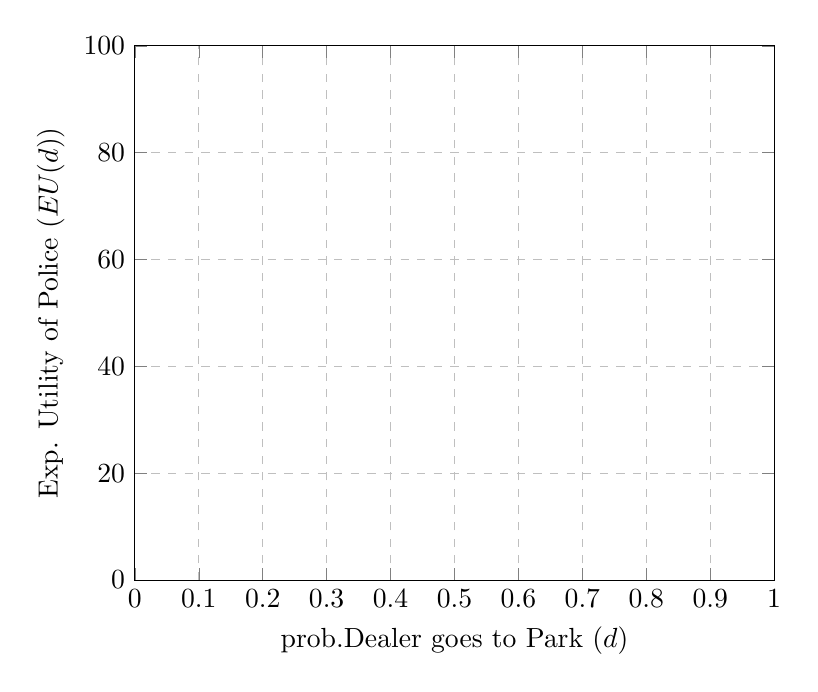
\begin{tikzpicture}
 
   \begin{axis}[
     width=0.8\textwidth,
     grid,
     xlabel={prob.Dealer goes to Park ($d$)},
     ylabel={Exp. Utility of Police ($EU(d)$)},
     xmin=0, xmax=1.0,
     ymin=0, ymax=100,
     xtick={0,.1,...,1.0},
     ytick={0,20,...,80,100},
     grid style=dashed,
     ]
 
     \addplot[draw=none] coordinates {(1,1)};
 
   \end{axis}
 \end{tikzpicture}

\end{frame}

\begin{frame}{Graph Drug Dealer's expected utilities}
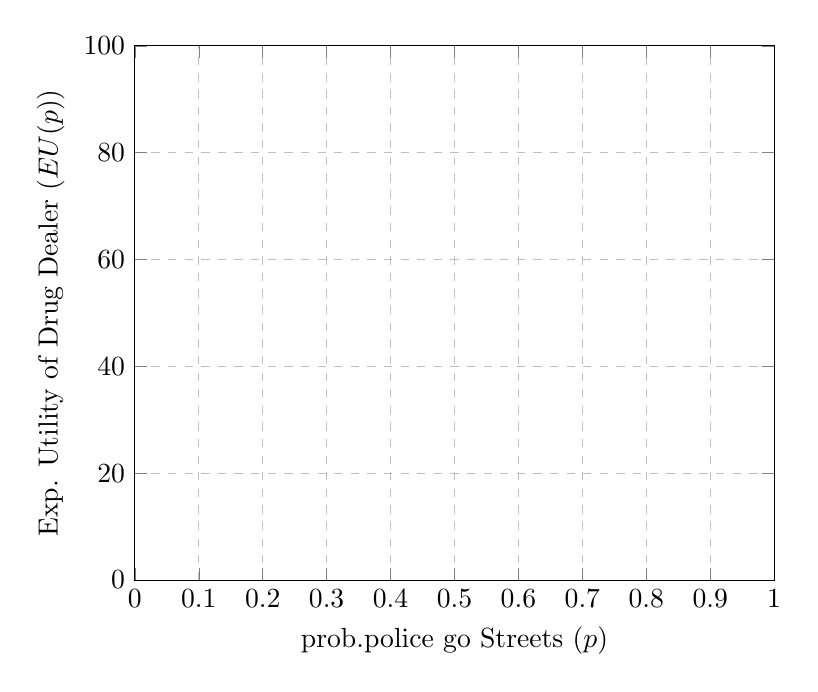
\begin{tikzpicture}
 
   \begin{axis}[
     width=0.8\textwidth,
     grid,
     xlabel={prob.police go Streets ($p$)},
     ylabel={Exp. Utility of Drug Dealer ($EU(p)$)},
     xmin=0, xmax=1.0,
     ymin=0, ymax=100,
     xtick={0,.1,...,1.0},
     ytick={0,20,...,80,100},
     grid style=dashed,
     ]
 
     \addplot[draw=none] coordinates {(1,1)};
 
   \end{axis}
 \end{tikzpicture}

\end{frame}

\begin{frame}{Graph Best Response functions}
 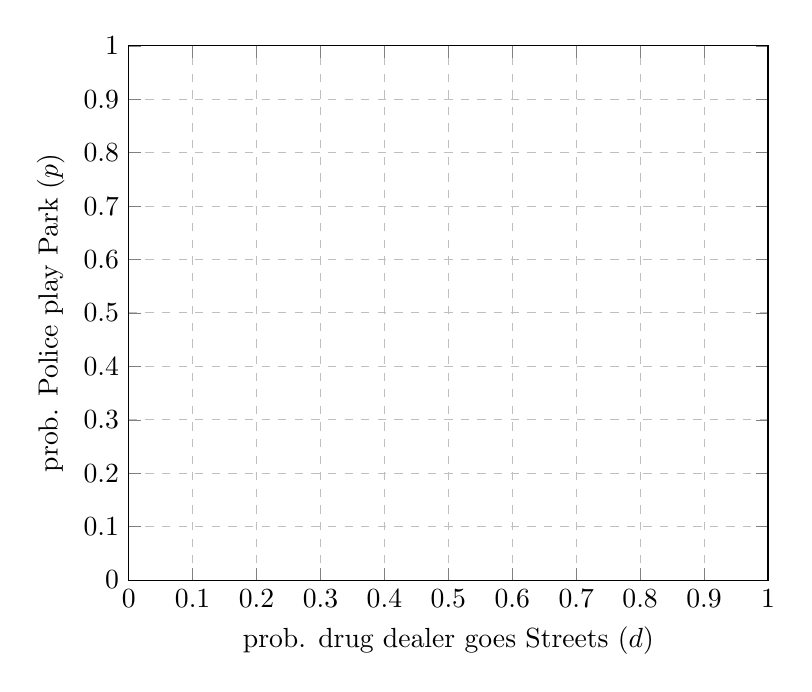
\begin{tikzpicture}
 
   \begin{axis}[
     width=0.8\textwidth,
     grid,
     xlabel={prob. drug dealer goes Streets ($d$)},
     ylabel={prob. Police play Park ($p$)},
     xmin=0, xmax=1.0,
     ymin=0, ymax=1.0,
     xtick={0,.1,...,1.0},
     ytick={0,.1,...,1.0},
     grid style=dashed,
     ]
 
     \addplot[draw=none] coordinates {(1,1)};
 
   \end{axis}
 \end{tikzpicture}
\end{frame}

\begin{frame}
\frametitle{MSNE in Patrol and Trade game:}
\begin{itemize}
\item When is the Police Officer indifferent between going to the Park and going to the Streets?
  \vspace{15mm}

\item When is the Drug Dealer indifferent between going to the Park and going to the Streets?
  \vspace{15mm}

  \item What is the \alert{Mixed Strategies Nash equilibrium?}
  \vspace{15mm}

\end{itemize}
\end{frame}

\begin{frame}{MSNE in Patrol and Trade game:}
\begin{itemize}
\item Note that the players' asymmetric preferences result in each of them buying a ticket for their more preferred concert most of the time in this MSNE.
\item If we gave them stronger preferences (i.e. increased the amount by which they prefer their favorite composer), it would amplify this effect in the MSNE.
\end{itemize}
\end{frame}

\begin{frame}
\frametitle{iClicker Q1}
\begin{itemize}
\item Consider the following game table. What are Player 1's expected payoffs, given Player 2's mixed strategy?
\end{itemize}
\begin{table}[h]
\centering
\begin{tabular}{cc|c|c|}
	& \multicolumn{1}{c}{} & \multicolumn{2}{c}{Player 2}\\
	& \multicolumn{1}{c}{} & \multicolumn{1}{c}{$Up (q)$}  & \multicolumn{1}{c}{$Down (1 - q)$} \\\cline{3-4}
	\multirow{2}*{Player 1}  & $Up (p)$ & 2, -2 & -3, 3 \\\cline{3-4}
	& $Down (1 - p)$ & -5, 5 & 1, -1 \\\cline{3-4}
\end{tabular}
\end{table}
  \begin{enumerate}[(a)]
\item $U_1(Up) = 5q - 3, U_1(Down) = 1 - 6q$
\item $U_1(Up) = 3 - 5q, U_1(Down) = 6q - 1$
\item $U_1(Up) = 5 - 7q, U_1(Down) = 1 - 6p$
\item $U_1(Up) = 7p - 5, U_1(Down) = 1 - 4p$
\item $U_1(Up) = 5 - 7p, U_1(Down) = 4p - 1$
\end{enumerate}
\end{frame}

\begin{frame}
\frametitle{iClicker Q2}
\begin{itemize}
\item Consider the following game table. What are \textbf{Player 2's} expected payoffs, given Player 1's mixed strategy?
\end{itemize}
\begin{table}[h]
\centering
\begin{tabular}{cc|c|c|}
& \multicolumn{1}{c}{} & \multicolumn{2}{c}{Player 2}\\
& \multicolumn{1}{c}{} & \multicolumn{1}{c}{$Up (q)$}  & \multicolumn{1}{c}{$Down (1 - q)$} \\\cline{3-4}
\multirow{2}*{Player 1}  & $Up (p)$ & 2, -2 & -3, 3 \\\cline{3-4}
& $Down (1 - p)$ & -5, 5 & 1, -1 \\\cline{3-4}
\end{tabular}
\end{table}
\begin{enumerate}[(a)]
\item $U_2(Up) = 5q - 3, U_2(Down) = 1 - 6q$
\item $U_2(Up) = 3 - 5q, U_2(Down) = 6q - 1$
\item $U_2(Up) = 5 - 7q, U_2(Down) = 1 - 6p$
\item $U_2(Up) = 7p - 5, U_2(Down) = 1 - 4p$
\item $U_2(Up) = 5 - 7p, U_2(Down) = 4p - 1$
\end{enumerate}
\end{frame}

\begin{frame}
\frametitle{iClicker Q3}
\begin{itemize}
\item The correct answers to the previous two questions were:
\begin{itemize}
\item $U_1(Up) = 5q - 3, U_1(Down) = 1 - 6q$.
\item $U_2(Up) = 5 - 7p, U_2(Down) = 4p - 1$.
\end{itemize}
\item Based on this, what are $p$ and $q$ in the MSNE of this game?
\begin{enumerate}[(a)]
\item $p^* = 4/11, \ q^* = 5/11$
\item $p^* = 4/11, \ q^* = 6/11$
\item $p^* = 6/11, \ q^* = 4/11$
\item $p^* = 7/11, \ q^* = 5/11$
\item $p^* = 7/11, \ q^* = 6/11$
\end{enumerate}
\end{itemize}
\end{frame}

\begin{frame}
\frametitle{An MSNE With Only One Mixed Strategy}
\begin{itemize}
	\item Consider the following game table:
\end{itemize}
\begin{table}[h]
	\centering
	\begin{tabular}{cc|c|c|}
		& \multicolumn{1}{c}{} & \multicolumn{2}{c}{Player 2}\\
		& \multicolumn{1}{c}{} & \multicolumn{1}{c}{$X~(q)$}  & \multicolumn{1}{c}{$Y~(1 - q)$} \\\cline{3-4}
		\multirow{2}*{Player 1}  & $A~(p)$ & 2, 2 & 3, 2 \\\cline{3-4}
		& $B~(1 - p)$ & 4, 3 & 0, 0 \\\cline{3-4}
	\end{tabular}
\end{table}
\begin{itemize}
	\item The players' expected payoffs are:
	\begin{itemize}
		\item $U_1(A) = 2q + 3(1 - q) = 2q + 3 - 3q = 3 - q$.
		\item $U_1(B) = 4q + 0(1 - q) = 4q$.
		\item $U_2(X) = 2p + 3(1 - p) = 2p + 3 - 3p = 3 - p$.
		\item $U_2(Y) = 2p + 0(1 - p) = 2p$.
	\end{itemize}
\end{itemize}
\end{frame}

\begin{frame}
\frametitle{An MSNE With Only One Mixed Strategy}
\begin{itemize}
\item Based on this, the conditions under which each player will use a mixed strategy are:
\end{itemize}
\begin{align*}
Player~1: && Player~2:&\\
3 - q &= 4q & 3 - p &= 2p\\
3 &= 5q & 3 &= 3p\\
q &= 3/5 & p &= 1
\end{align*}
\begin{itemize}
\item We've never seen anything like $p = 1$ in this context before...
\item $p = 1$ tells us that Player 2 will only play a mixed strategy
  if Player 1 only play A, which isn't really a mixed strategy at all.
\item This usually occurs when one strategy \textbf{weakly} dominates another.
\end{itemize}
\end{frame}

\begin{frame}
\frametitle{An MSNE With Only One Mixed Strategy}
\begin{itemize}
	\item We can still approach this the same way that we have in the past:
	\item Suppose that in the MSNE, Player 1 plays a (non-trivial) mixed strategy. Then Player 2 must also play a mixed strategy, in which q = 3/5.
	\begin{itemize}
		\item But Player 2 will only play a mixed strategy if Player 1 plays the mixed strategy where p = 1...which is a trivial mixed strategy. This is a contradiction, and it means that there is no MSNE where Player 1 plays a non-trivial mixed strategy.
	\end{itemize}
\end{itemize}
\end{frame}

\begin{frame}
\frametitle{An MSNE With Only One Mixed Strategy}
\begin{itemize}
\item Approach it the other way next: Suppose Player 2 plays a non-trivial mixed strategy. Then Player 1 must play A as a pure strategy.
\begin{itemize}
	\item Player 2 will play A if $3 - q \geq 4q$, i.e. if $3/5 \geq q$.
\end{itemize}
\item This lets Player 2 play a non-trivial mixed strategy! There is no contradiction here.
\end{itemize}
\end{frame}

\begin{frame}{An MSNE with only one mixed strategy}
\begin{itemize}
\item There are a range of MSNEs here: all strategy profiles of the form \{(1, 0), (q, 1 - q)\}, in which $q \in (0, 3/5]$, are MSNEs.
\item There are also two trivial MSNEs, \{(1, 0), (0, 1)\} and \{(0, 1), (1, 0)\}, which are really just the pure-strategy Nash equilibria (A, Y) and (B, X) expressed in the form of an MSNE.
\item It will help to understand what's going on with the Best Responses graph:
\end{itemize}
\end{frame}

\begin{frame}{Graph Best Responses}
  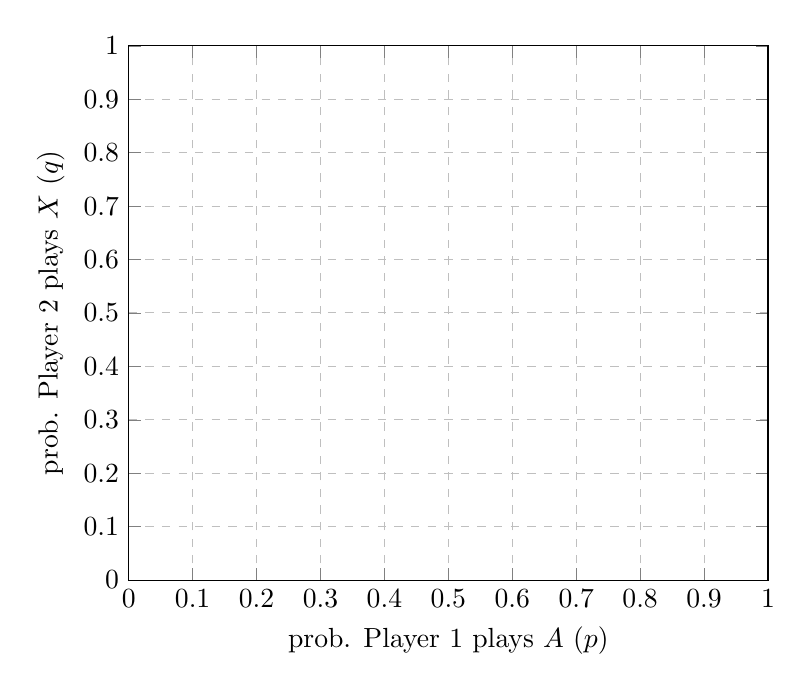
\begin{tikzpicture}
 
   \begin{axis}[
     width=0.8\textwidth,
     grid,
     xlabel={prob. Player 1 plays $A$ ($p$)},
     ylabel={prob. Player 2 plays $X$ ($q$)},
     xmin=0, xmax=1.0,
     ymin=0, ymax=1.0,
     xtick={0,.1,...,1.0},
     ytick={0,.1,...,1.0},
     grid style=dashed,
     ]
 
     \addplot[draw=none] coordinates {(1,1)};
 
   \end{axis}
 \end{tikzpicture}
 
\end{frame}

\begin{frame}
\frametitle{Absence of MSNEs}
\begin{itemize}
	\item Let us return to the Prisoner's Dilemma and check for MSNEs:
\end{itemize}
\begin{table}[h]
	\centering
	\begin{tabular}{cc|c|c|}
		& \multicolumn{1}{c}{} & \multicolumn{2}{c}{Luca}\\
		& \multicolumn{1}{c}{} & \multicolumn{1}{c}{$Testify~(q)$}  & \multicolumn{1}{c}{$Keep~Quiet~(1-q)$} \\\cline{3-4}
		\multirow{2}*{Guido}  & $Testify~(p)$ & $-10,-10$ & $0,-20$ \\\cline{3-4}
		& $Keep~Quiet~(1-p)$ & $-20,0$ & $-1,-1$ \\\cline{3-4}
	\end{tabular}
\end{table}
\begin{itemize}
	\item Guido and Luca's expected payoffs are:
	\begin{itemize}
		\item $U_G(Testify) = -10q + 0(1 - q) = -10q$.
		\item $U_G(Keep Quiet) = -20q + (-1)(1 - q) = -1 - 19q$.
		\item $U_L(Testify) = -10p + 0(1 - p) = -10p$.
		\item $U_L(Keep Quiet) = -20p + (-1)(1 - p) = -1 - 19p$.
	\end{itemize}
\end{itemize}
\end{frame}

\begin{frame}
\frametitle{Absence of MSNEs}
\begin{itemize}
\item Guido will play a mixed strategy if:
\end{itemize}
\begin{align*}
-10q &= -1 - 19q\\
9q &= -1\\
q &= -1/9
\end{align*}
\begin{itemize}
  \item But \textbf{-1/9 is not a valid probability!}
\item We could also note that if $q\in [0, 1]$, which is the range for valid probabilities, $-10q$ is always greater than $-1 - 19q$. In other words, as we saw weeks ago, $Testify$ strictly dominates $Keep~Quiet$...so why would Guido mix between the two of them?
\end{itemize}
\end{frame}

\begin{frame}
\frametitle{Getting Bad Probabilities}
\begin{itemize}
	\item If you've set up the expected-payoff equation, and solved for a player's mixed strategy, and you find that the probability is less than 0, or more than 1...
	\item \textbf{It means something is wrong.} Probability can only be between 0 and 1 (inclusive).
	\item First of all, double-check your math---it could be an algebra error.
	\item But if you're confident in your math, this means that there is \textbf{no way that the player would ever play a mixed strategy}: in fact, they have a strictly dominated strategy.
	\item There will be no MSNE where this player uses a mixed strategy---but there might be MSNEs where the other player does, so you should still check that.
\end{itemize}
\end{frame}

\begin{frame}
\frametitle{MSNE in a Larger Game}
\begin{itemize}
	\item Suppose that we have this 3$\times$2 game:
\end{itemize}
\begin{table}[h]
\centering
\begin{tabular}{cr|c|c|}
	& \multicolumn{1}{c}{} & \multicolumn{2}{c}{Player 2}\\
	& \multicolumn{1}{c}{} & \multicolumn{1}{c}{X (r)}  & \multicolumn{1}{c}{Y (1 - r)} \\\cline{3-4}
	\multirow{3}*{Player 1}  & A (p) & 2, 1 & 0, 1 \\\cline{3-4}
	& B (q) & 1, 2 & 2, 0 \\\cline{3-4}
	& C (1 - p - q) & 0, 0 & 3, 2 \\\cline{3-4}
\end{tabular}
\end{table}
\begin{itemize}
	\item First, note that in this game, Player 1's mixed strategy uses probabilities p, q, and 1 - p - q, since they have three pure strategies.
	\item As a rule of thumb, a player's mixed strategy will need one variable less than their number of strategies.
\end{itemize}
\end{frame}

\begin{frame}{Existence of Nash Equilibria}
  What is the \textit{pure strategy} Nash Equilibria of the game
  \alert{Rock, Paper, Scissors}?
\end{frame}

\begin{frame}{Existence of Nash Equilibria}
  What is the \textbf{Mixed Strategy Nash Equilibria} of the game
  \alert{Rock, Paper, Scissors}?
\end{frame}

\begin{frame}{Existence of Nash equilibria}
  Any with game with a \textit{finite} set of moves
  will have at least one \textbf{Nash equilibrium}
  when allowing for \textit{mixed strategies}.

  The true power of this concept and the most important 
  contribution of its namesake, John Nash,
  is that it is a simple concept which has universal application.
\end{frame}

\begin{frame}{Existence of Nash equilibria}
\frametitle{MSNE in a Larger Game}
\begin{itemize}
	\item To begin with, let's put together Player 1's expected payoffs, of which there will be three:
	\begin{itemize}
		\item $U_1(A) = 2r + 0 = 2r$.
		\item $U_1(B) = 1r + 2(1 - r) = 2 - r$.
		\item $U_1(C) = 0 + 3(1 - r) = 3 - 3r$.
	\end{itemize}
	\item Next, let's see what it would take to get Player 1 to mix different pairs of strategies:
	\begin{itemize}
		\item A and B: $2r = 2 - r \implies r = \frac{2}{3}$.
		\item A and C: $2r = 3 - 3r \implies r = \frac{3}{5}$.
		\item B and C: $2 - r = 3 - 3r \implies r = \frac{1}{2}$.
	\end{itemize}
	\item Note that each pair of strategies requires a different value of $r$: there is no mixed strategy for Player 2 that would make Player 1 willing to mix all three of their pure strategies.
\end{itemize}
\end{frame}

\begin{frame}
\frametitle{MSNE in a Larger Game}
\begin{itemize}
	\item Let's check Player 2's expected payoffs next:
	\begin{itemize}
		\item $U_2(X) = 1p + 2q + 0$.
		\item $U_2(Y) = 1p + 0 + 2(1 - p - q)$.
	\end{itemize}
	\item So Player 2 will play a mixed strategy if $p + 2q = p + 2(1 - p - q) \implies q = 1 - p - q$.
	\item There are two ways that this can be true: Either Player 1 plays B and C with equal probability (and we know from earlier that they would \textbf{only} be playing these two, not A), or Player 1 plays A only, and B and C not at all. 
\end{itemize}
\end{frame}

\begin{frame}
\frametitle{MSNE in a Larger Game}
\begin{itemize}
	\item So, one type of MSNE is where Player 1 only plays A: this requires $2r \geq 2 - r$ and $2r \geq 3 - 3r$, which imply that $r \geq \frac{2}{3}$ and $r \geq \frac{3}{5}$.
	\begin{itemize}
		\item MSNE: \{(1, 0, 0), (r, 1 - r)\}, where $r \geq \frac{2}{3}$.
	\end{itemize}
	\item And the other type of MSNE is where Player 1 plays B and C with equal (1/2) probability, and Player 2 plays X and Y with equal (1/2) probability.
	\begin{itemize}
		\item MSNE: \{(0, 1/2, 1/2), (1/2, 1/2)\}
	\end{itemize}
\end{itemize}
\end{frame}



\section{Advanced Mixed Strategies}


\begin{frame}
\frametitle{MSNE in a Larger Game}
\begin{itemize}
	\item Suppose that we have this 3$\times$2 game:
\end{itemize}
\begin{table}[h]
\centering
\begin{tabular}{cr|c|c|}
	& \multicolumn{1}{c}{} & \multicolumn{2}{c}{Player 2}\\
	& \multicolumn{1}{c}{} & \multicolumn{1}{c}{X (r)}  & \multicolumn{1}{c}{Y (1 - r)} \\\cline{3-4}
	\multirow{3}*{Player 1}  & A (p) & 2, 1 & 0, 1 \\\cline{3-4}
	& B (q) & 1, 2 & 2, 0 \\\cline{3-4}
	& C (1 - p - q) & 0, 0 & 3, 2 \\\cline{3-4}
\end{tabular}
\end{table}
\begin{itemize}
	\item Player 1's mixed strategy uses probabilities p, q, and 1 - p - q, since they have three pure strategies.
\end{itemize}
\end{frame}

% - - - - - - - - - - - - - - - - - - - - - - - - - - - - - - - - - - - - - - -

\begin{frame}{Existence of Nash equilibria}
\frametitle{MSNE in a Larger Game}
\begin{itemize}
	\item Algebraically:
	\begin{itemize}
		\item $U_1(A) = 2r + 0 = 2r$.
		\item $U_1(B) = 1r + 2(1 - r) = 2 - r$.
		\item $U_1(C) = 0 + 3(1 - r) = 3 - 3r$.
	\end{itemize}
	\end{itemize}
\end{frame}

% - - - - - - - - - - - - - - - - - - - - - - - - - - - - - - - - - - - - - - -

\begin{frame}{Graph Player 1's expected utilities}
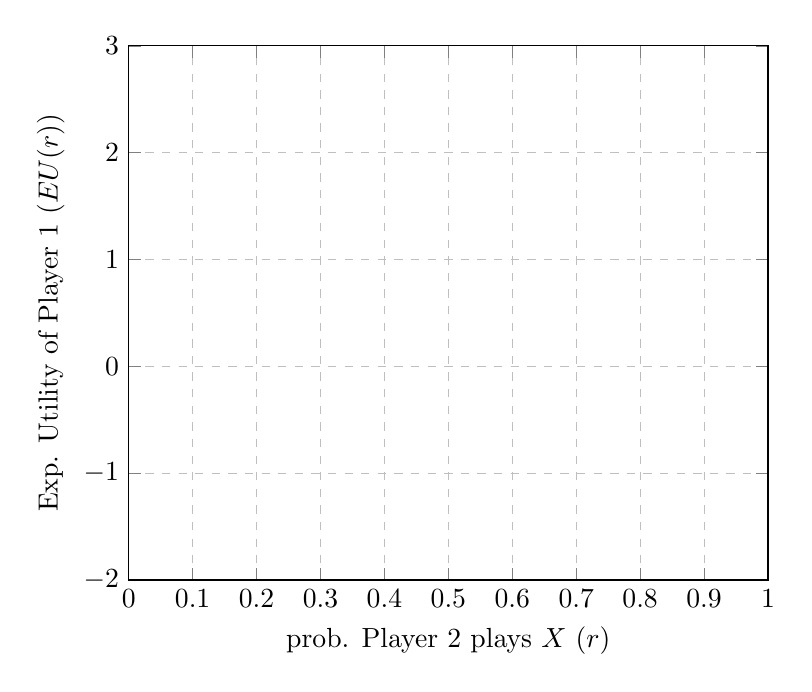
\begin{tikzpicture}
 
   \begin{axis}[
     width=0.8\textwidth,
     grid,
     xlabel={prob. Player 2 plays $X$ ($r$) },
     ylabel={Exp. Utility of Player 1 ($EU(r)$)},
     xmin=0, xmax=1.0,
     ymin=-2, ymax=3,
     xtick={0,.1,...,1.0},
     ytick={-2, -1, 0, 1, 2, 3},
     grid style=dashed,
     ]
 
     \addplot[draw=none] coordinates {(1,1)};
   \end{axis}
 \end{tikzpicture}
\end{frame}

% - - - - - - - - - - - - - - - - - - - - - - - - - - - - - - - - - - - - - - -

\begin{frame}{When will Player 1 mix?}
  \begin{itemize}
    \item What it would take to get Player 1 to mix different pairs of strategies:
	\begin{itemize}
		\item A and B: $2r = 2 - r \implies r = \frac{2}{3}$.
		\item A and C: $2r = 3 - 3r \implies r = \frac{3}{5}$.
		\item B and C: $2 - r = 3 - 3r \implies r = \frac{1}{2}$.
	\end{itemize}

    \item Note that there is no intersection between all three lines simultaneously

    \item This means that Player 1 will never mix between all three strategies
  \end{itemize}
\end{frame}

% - - - - - - - - - - - - - - - - - - - - - - - - - - - - - - - - - - - - - - -

\begin{frame}
\frametitle{MSNE in a Larger Game}
\begin{itemize}
	\item Let's check Player 2's expected payoffs next:
	\begin{itemize}
		\item $U_2(X) = 1p + 2q + 0$.
		\item $U_2(Y) = 1p + 0 + 2(1 - p - q)$.
	\end{itemize}
	\item So Player 2 will play a mixed strategy if
  $$p + 2q = p + 2(1 - p - q)$$ 
  $$\implies q = 1 - p - q$$.

  \begin{itemize}
    \item Recall that $q$ was the probability we put on Player 2 playing $B$,
    \item and $1-p-q$ was the probability they play $C$. 
  \end{itemize}

\end{itemize}
\end{frame}

% - - - - - - - - - - - - - - - - - - - - - - - - - - - - - - - - - - - - - - -

\begin{frame}{visualizing Player 2's Best Responses}
  \begin{center}
  \begin{tikzpicture}
    \draw (0,0) coordinate[label=below:$A$] (a) --
    (5,0) coordinate[label=below:$C$] (c) --
    (2.5, 4.3) coordinate[label=above:$B$] (b) -- cycle ;
  \end{tikzpicture}
  \end{center}
\end{frame}

% - - - - - - - - - - - - - - - - - - - - - - - - - - - - - - - - - - - - - - -

\begin{frame}{When will Player 2 mix?}
  \begin{itemize}
    \item We found they are indifferent between $X$ and $Y$ when 
    $$ q = 1 - p - d $$.

	  \item There are two ways that this can be true: 
    \begin{itemize}
      \item Either Player 1 plays B and C with equal probability
      (and we know from earlier that they would \textbf{only} be playing these two, not A),
      \item or Player 1 plays A only, and B and C not at all. 
    \end{itemize}
  \end{itemize}
\end{frame}

% - - - - - - - - - - - - - - - - - - - - - - - - - - - - - - - - - - - - - - -

\begin{frame}
\frametitle{MSNE in a Larger Game}
\underline{Case 1}: Player 1 only plays A:
\begin{itemize}
  \item this requires $2r \geq 2 - r$ and $2r \geq 3 - 3r$,
  \item which imply that $r \geq \frac{2}{3}$ and $r \geq \frac{3}{5}$.
  \item \textbf{MSNE 1:} \{(1, 0, 0), (r, 1 - r)\}, where $r \geq \frac{2}{3}$.
	\end{itemize}
\end{frame}

% - - - - - - - - - - - - - - - - - - - - - - - - - - - - - - - - - - - - - - -

\begin{frame}{MSNE in a Larger Game}
\underline{Case 2}: Player 1 plays $B$ and $C$ with equal probability 
  \begin{itemize}
   \item then Player 2 plays X and Y with equal (1/2) probability.
    \item \textbf{MSNE}: \{(0, 1/2, 1/2), (1/2, 1/2)\}
  \end{itemize} 
\end{frame}

% - - - - - - - - - - - - - - - - - - - - - - - - - - - - - - - - - - - - - - -

\begin{frame}{What about a 3x3 game?}
\begin{table}[h]
\centering
  \begin{tabular}{cr|c|c|c|}
	& \multicolumn{1}{c}{} & \multicolumn{3}{c}{Player 2}\\
    & \multicolumn{1}{c}{} & Rock ($r_2$) & Paper ($p_2$) & Scissors ($1-r_2-p_2$) \\\cline{3-5}
    \multirow{3}*{Player 1}  & Rock ($r_1$) & 0, 0 & -1, 1 & 1, -1 \\\cline{3-5}
    & Paper ($p_1$) & 1, -1 & 0,0 & -1, 1 \\\cline{3-5}
    & Scissors  & -1, 1 & 1, -1 & 0, 0 \\\cline{3-5}
\end{tabular}
\end{table}
\end{frame}

% - - - - - - - - - - - - - - - - - - - - - - - - - - - - - - - - - - - - - - -

\begin{frame}{What about a 3x3 game?}
  \begin{itemize}
    \item Rock, Paper, Scissors is a \textit{symmetric} game, so let's just pay attention to Player 1's utility 

    \item $EU_1(Rock | r_2, p_2) = $

    \item $EU_1(Paper | r_2, p_2) = $

    \item $EU_1(Scissors | r_2, p_2) = $
  \end{itemize}
  
\end{frame}

\begin{frame}{visualizing Player 1's Best Responses}
  \begin{center}
  \begin{tikzpicture}
    \draw (0,0) coordinate[label=below:$Rock$] (r) --
    (8,0) coordinate[label=below:$Paper$] (p) --
    (4, 7) coordinate[label=above:$Scissors$] (s) -- cycle ;
  \end{tikzpicture}
  \end{center}
\end{frame}

% - - - - - - - - - - - - - - - - - - - - - - - - - - - - - - - - - - - - - - -

\begin{frame}{Finding MSNE in 3x3 game}
  \begin{minipage}{0.45\textwidth}
  \begin{center}
  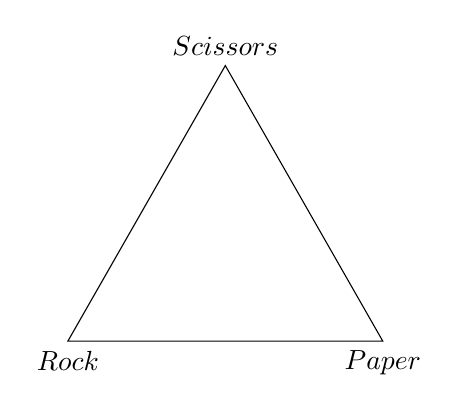
\begin{tikzpicture}
    \draw (0,0) coordinate[label=below:$Rock$] (r) --
    (4,0) coordinate[label=below:$Paper$] (p) --
    (2, 3.5) coordinate[label=above:$Scissors$] (s) -- cycle ;
  \end{tikzpicture}
  \end{center}
  \end{minipage} 
  \begin{minipage}{0.45\textwidth}
  \begin{center}
  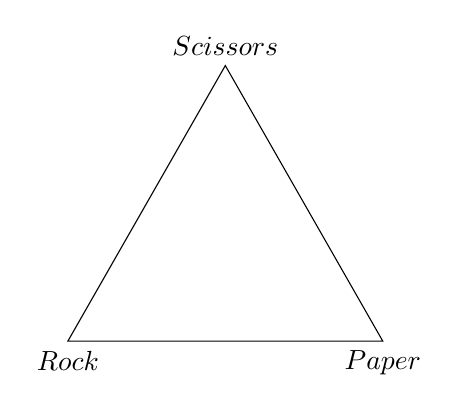
\begin{tikzpicture}
    \draw (0,0) coordinate[label=below:$Rock$] (r) --
    (4,0) coordinate[label=below:$Paper$] (p) --
    (2, 3.5) coordinate[label=above:$Scissors$] (s) -- cycle ;
  \end{tikzpicture}
  \end{center}
  \end{minipage} 
\end{frame}

% - - - - - - - - - - - - - - - - - - - - - - - - - - - - - - - - - - - - - - -

\begin{frame}{Finding MSNE in 3x3 game}
  So the results from our math confirm our intuition that the stable strategies in equilibrium are:
  \begin{itemize}
    \item Player 1 plays Rock with $r=1/3$, Paper with $p=1/3$, and Scissors with
    $1-p-r=1/3$
    \item Player 1 plays Rock with $r=1/3$, Paper with $p=1/3$, and Scissors with
    $1-p-r=1/3$
  \end{itemize}
\end{frame}

% - - - - - - - - - - - - - - - - - - - - - - - - - - - - - - - - - - - - - - -

\begin{frame}{Another 3x3 game}
 \begin{table}[h]
\centering
  \begin{tabular}{cr|c|c|c|}
	& \multicolumn{1}{c}{} & \multicolumn{3}{c}{Player 2}\\
    & \multicolumn{1}{c}{}            &  Left  & Center & Right  \\\cline{3-5}
    \multirow{3}*{Player 1}  & Top    &  2,  1 &  3,  0 &  3,  0 \\\cline{3-5}
                             & Middle &  3,  0 &  0,  1 &  3,  0 \\\cline{3-5}
                             & Bottom &  3,  0 &  3,  0 &  2,  1 \\\cline{3-5}
\end{tabular}
\end{table}
\end{frame}

% - - - - - - - - - - - - - - - - - - - - - - - - - - - - - - - - - - - - - - -

\begin{frame}{Solving for 3-strategy MSNE}
  \textbf{Step 1:} Define Mixed Strategies
  \begin{itemize}

    \item \underline{Player 1's mixed strategy:} 
    Let $\sigma_1 = (t, m, b)$  

    \item \underline{Player 2's mixed strategy:} 
    Let $\sigma_2 = (\ell, c, r)$  

  \end{itemize}
  
  Note that the lowercase letters represent the probabilities played
  on the uppercase pure strategies.
\end{frame}

% - - - - - - - - - - - - - - - - - - - - - - - - - - - - - - - - - - - - - - -

\begin{frame}{Solving for 3-strategy MSNE}
  \textbf{Step 2:} Solve for Expected Utilities

  \begin{multicols}{2}
  \begin{minipage}{.5\textwidth}
  \begin{itemize}
    
    \item \underline{Player 1:}
    \begin{itemize}

      \item $EU_1(T, \sigma_2) = $
      \vspace{8mm}

      \item $EU_1(M, \sigma_2) = $
      \vspace{8mm}

     \item $EU_1(B, \sigma_2) = $
      \vspace{8mm}
      
    \end{itemize}
  \end{itemize}
  \end{minipage}

  \begin{minipage}{.5\textwidth}
  \begin{itemize}
    
    \item \underline{Player 2:}
    \begin{itemize}

      \item $EU_2(L, \sigma_1) = $
      \vspace{8mm}
      \item $EU_2(C, \sigma_1) = $
      \vspace{8mm}
      \item $EU_2(R, \sigma_1) = $
      \vspace{8mm}
      
    \end{itemize}
  \end{itemize}
  \end{minipage}
  \end{multicols}

\end{frame}

% - - - - - - - - - - - - - - - - - - - - - - - - - - - - - - - - - - - - - - -

\begin{frame}{Solving for 3-strategy MSNE}
  \textbf{Step 3:} Find Indifference Conditions
  \begin{itemize}

    \item \underline{When will Player 1 mix between 2 pure strategies?} 
    \begin{itemize}
      \item When does $EU_1(Top, \sigma_2) = EU_1(Middle, \sigma_2)$:
      \vspace{14mm}
      \item When does $EU_1(Top, \sigma_2) = EU_1(Bottom, \sigma_2)$:
      \vspace{14mm}
      \item When does $EU_1(Middle, \sigma_2) = EU_1(Bottom, \sigma_2)$:
      \vspace{14mm}
      
    \end{itemize}
    
  \end{itemize}
  
\end{frame}

% - - - - - - - - - - - - - - - - - - - - - - - - - - - - - - - - - - - - - - -

\begin{frame}{Solving for 3-strategy MSNE}
  \textbf{Step 3:} Find Indifference Conditions
  \begin{itemize}

    \item \underline{When will Player 2 mix between 2 pure strategies?} 
    \begin{itemize}
      \item When does $EU_2(Left, \sigma_1) = EU_2(Center, \sigma_1)$:
      \vspace{14mm}
      \item When does $EU_2(Left, \sigma_1) = EU_2(Right, \sigma_1)$:
      \vspace{14mm}
      \item When does $EU_2(Center, \sigma_1) = EU_2(Right, \sigma_1)$:
      \vspace{14mm}
      
    \end{itemize}
    
  \end{itemize}
  
\end{frame}

% - - - - - - - - - - - - - - - - - - - - - - - - - - - - - - - - - - - - - - -

\begin{frame}{Solving for 3-strategy MSNE}
  \textbf{Step 4.a:} Graph Indifference Points on Number Lines for Player 1

  \vspace{60mm}
  
\end{frame}

% - - - - - - - - - - - - - - - - - - - - - - - - - - - - - - - - - - - - - - - 

\begin{frame}{Solving for 3-strategy MSNE}
  \textbf{Step 4.b:} Combine Number Lines into Player 1's BR Triangle
  \begin{center}
  \begin{tikzpicture}
    \draw (0,0) coordinate[label=below:Left] (r) --
    (6,0) coordinate[label=below:Right] (p) --
    (3, 5) coordinate[label=above:Center] (s) -- cycle ;
  \end{tikzpicture}
  \end{center}
\end{frame}

% - - - - - - - - - - - - - - - - - - - - - - - - - - - - - - - - - - - - - - - 

\begin{frame}{Solving for 3-strategy MSNE}
  \textbf{Step 4.c:} Graph Indifference Points on Number Lines for Player 2

  \vspace{60mm}
  
\end{frame}

% - - - - - - - - - - - - - - - - - - - - - - - - - - - - - - - - - - - - - - - 

\begin{frame}{Solving for 3-strategy MSNE}
  \textbf{Step 4.d:} Combine Number Lines into Player 2's BR Triangle
  \begin{center}
  \begin{tikzpicture}
    \draw (0,0) coordinate[label=below:Top] (r) --
    (6,0) coordinate[label=below:Bottom] (p) --
    (3, 5) coordinate[label=above:Middle] (s) -- cycle ;
  \end{tikzpicture}
  \end{center}
\end{frame}

% - - - - - - - - - - - - - - - - - - - - - - - - - - - - - - - - - - - - - - - 

\begin{frame}{Solving for 3-strategy MSNE}
  \textbf{Step 5:} Check Cases for possible Nash Equilibria:

  \vspace{60mm}
  
\end{frame}

% - - - - - - - - - - - - - - - - - - - - - - - - - - - - - - - - - - - - - - - 



\end{document}
